% !TEX TS-program = pdflatex
% !TEX encoding = UTF-8 Unicode

% This is a simple template for a LaTeX document using the "article" class.
% See "book", "report", "letter" for other types of document.

\documentclass[11pt]{article} % use larger type; default would be 10pt

\usepackage[utf8]{inputenc} % set input encoding (not needed with XeLaTeX)

%%% Examples of Article customizations
% These packages are optional, depending whether you want the features they provide.
% See the LaTeX Companion or other references for full information.

%%% PAGE DIMENSIONS
\usepackage{geometry} % to change the page dimensions
\geometry{a4paper} % or letterpaper (US) or a5paper or....
\geometry{margin=1in} % for example, change the margins to 2 inches all round
% \geometry{landscape} % set up the page for landscape
%   read geometry.pdf for detailed page layout information

\usepackage{graphicx} % support the \includegraphics command and options

% \usepackage[parfill]{parskip} % Activate to begin paragraphs with an empty line rather than an indent
\usepackage{amssymb}
\usepackage{amsmath}
%%% PACKAGES
\usepackage{booktabs} % for much better looking tables
\usepackage{array} % for better arrays (eg matrices) in maths
\usepackage{paralist} % very flexible & customisable lists (eg. enumerate/itemize, etc.)
\usepackage{verbatim} % adds environment for commenting out blocks of text & for better verbatim
\usepackage{subfig} % make it possible to include more than one captioned figure/table in a single float
% These packages are all incorporated in the memoir class to one degree or another...

%%% HEADERS & FOOTERS
\usepackage{fancyhdr} % This should be set AFTER setting up the page geometry
\pagestyle{fancy} % options: empty , plain , fancy
\renewcommand{\headrulewidth}{0pt} % customise the layout...
\lhead{}\chead{}\rhead{}
\lfoot{}\cfoot{\thepage}\rfoot{}

%%% SECTION TITLE APPEARANCE
\usepackage{sectsty}
\allsectionsfont{\sffamily\mdseries\upshape} % (See the fntguide.pdf for font help)
% (This matches ConTeXt defaults)

%%% ToC (table of contents) APPEARANCE
\usepackage[nottoc,notlof,notlot]{tocbibind} % Put the bibliography in the ToC
\usepackage[titles,subfigure]{tocloft} % Alter the style of the Table of Contents
\usepackage{bbm}
\usepackage{endnotes}

\renewcommand{\cftsecfont}{\rmfamily\mdseries\upshape}
\renewcommand{\cftsecpagefont}{\rmfamily\mdseries\upshape} % No bold!
\DeclareMathOperator*{\argmax}{arg\,max}
\DeclareMathOperator*{\argmin}{arg\,min}

\usepackage{graphicx}
\graphicspath{ {./pings/} }

\newcount\colveccount
\newcommand*\colvec[1]{
        \global\colveccount#1
        \begin{pmatrix}
        \colvecnext
}
\def\colvecnext#1{
        #1
        \global\advance\colveccount-1
        \ifnum\colveccount>0
                \\
                \expandafter\colvecnext
        \else
                \end{pmatrix}
        \fi
}

\newcommand{\norm}[1]{\left\lVert#1\right\rVert}

\title{Computational Problem Set 4}
\author{Michael B. Nattinger, Sarah J. Bass, Xinxin Hu}

\begin{document}
\maketitle
\section{Results}
First we present the transition path of the economy, then we present the EV-related measures.

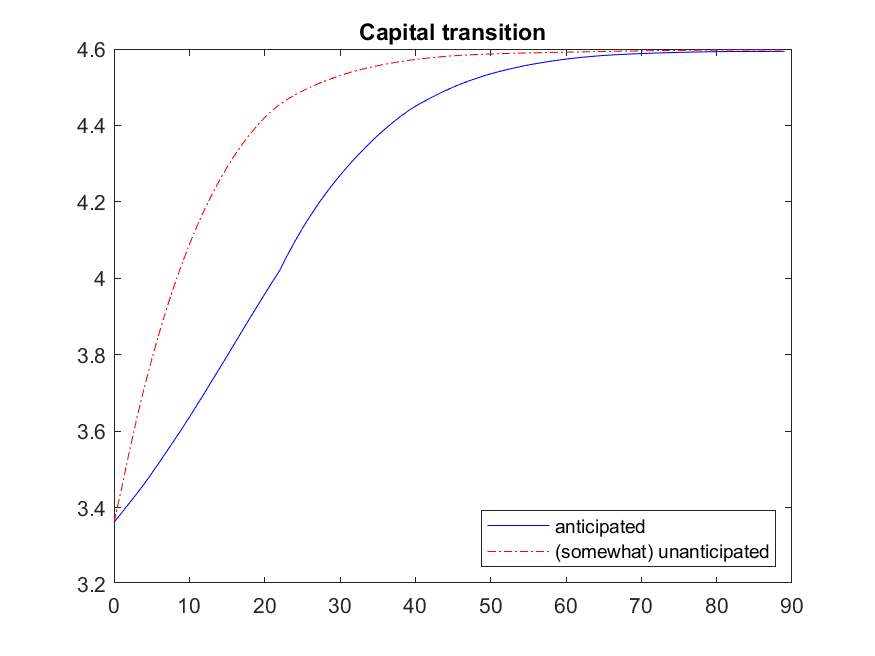
\includegraphics{k}

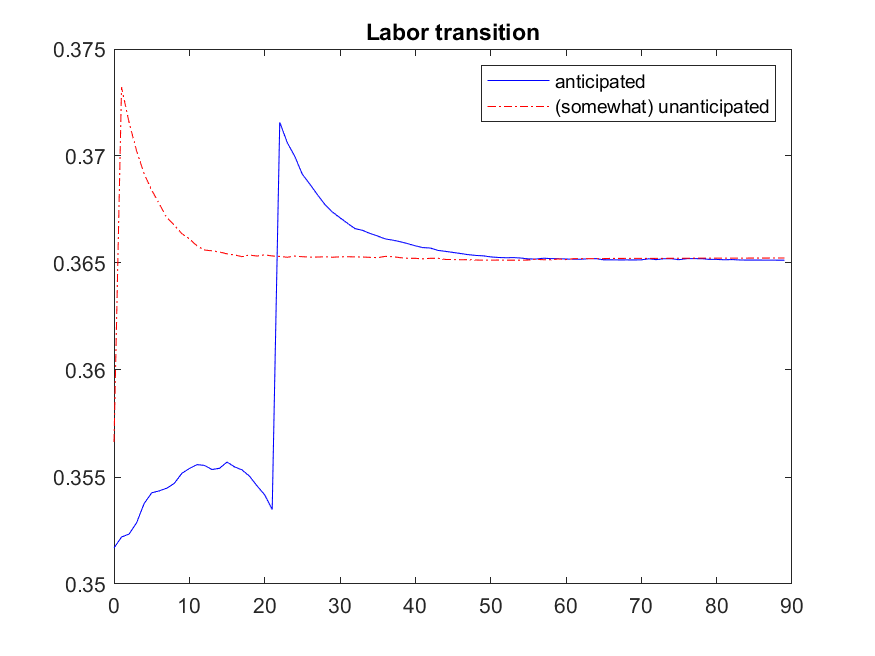
\includegraphics{l}

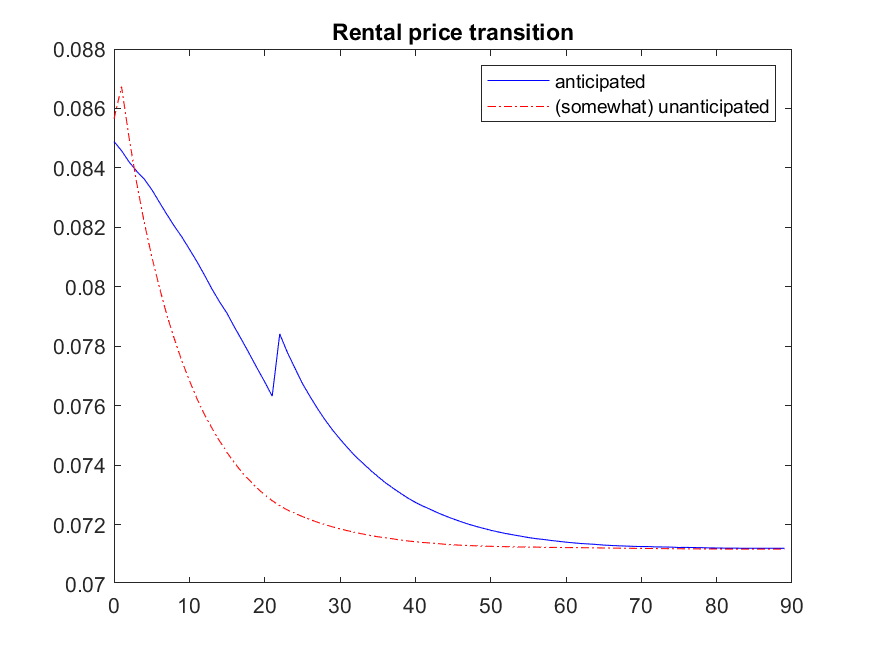
\includegraphics{r}

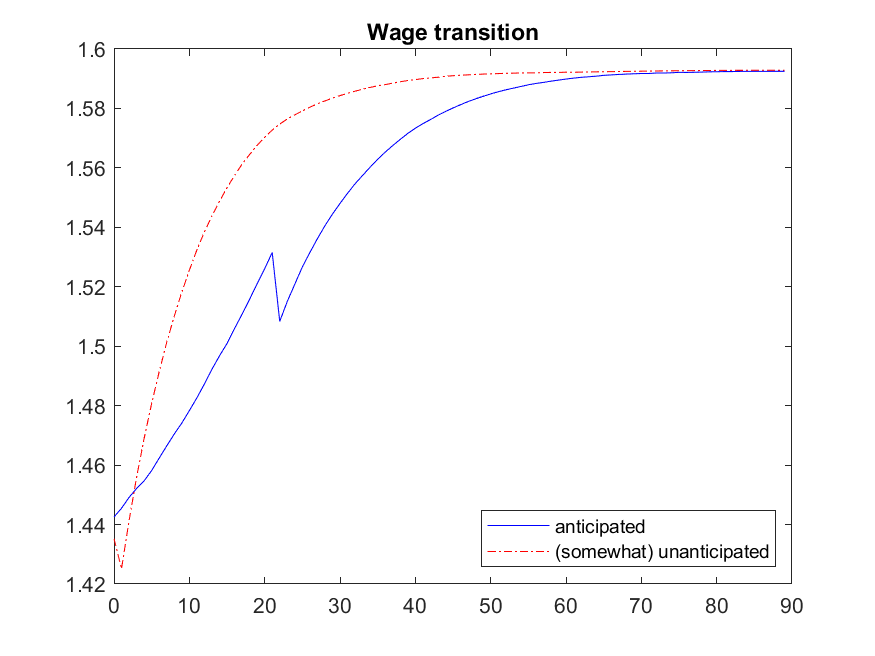
\includegraphics{w}

Our results show that capital adjusts gradually to the change, rising as households save precautionarily. Labor adjusts immediately in response to the news, as households work more to fund their increased capital investment. There is also a second spike at $t=1$ as the labor wedge is removed when the taxes change. The rental price increases immediately on impact due to the labor spike, and similarly wage falls on impact. Both variables experience a second spike from the removal of the labor wedge.  As the capital levels rise gradually, the rental price falls and the wage rises.

In the experiment where the switch occurs in a later period, we see that the short- and long-run effects are consistent qualitatively. The most significant difference is the transition point where the tax change occurs. This spike was occuring in period $t=1$ and now it is occuring later, at time $t=21$. In the capital transition, there is now a small kink in the capital transition.

\begin{center}
\begin{tabular}{ll}
& Equilibrium \\ 
\hline 
Capital & 5.0451 \\ 
Wage & 1.1461 \\ 
Interest rate & 0.12778 \\ 
\hline 
\end{tabular}
\end{center}

Our EV measure shows that the agents are substantially worse off, on average, due to the tax change. The agents are less worse off when the shock is anticipated. Voting numbers are consistent with this finding - most of the household mass is worse off in both cases, but fewer are worse off in the second experiment when the change is anticipated.

\end{document}
